\section{technische Umsetzung des Datenflusses zur Dashboardanzeige}
\label{ch:Dashboard:sec:Datenfluss}
Die Dashboard-Anzeige sitzt symbolisch gesprochen auf dem alten System (s. \autoref{ch:IST-Zustand:sec:Aufbau_altes_System}) auf. Das bedeutet, dass es die bestehenden Daten auswertet und diese neu darstellt (s. \autoref{fig:DB_Datenfluss}).

Die Daten werden von einem Parser eingelesen (s. \autoref{Add:Dashboard:Parser_Code}), welcher diese in Fehlerkategorien zusammenfasst (s. \autoref{ch:Dashboard:sec:Aufbau}) und im JSON-Format abspeichert (s. \autoref{Add:Dashboard:JSON}). Der Parser-Code wird regelmäßig durch einen Jenkins-Job aufgerufen und dessen Ausgabe auf einen Dateiserver gespeichert und die vorherige Datei überschrieben.

Das Dashboard kann auf den Server zugreifen und mithilfe der API über den Adress-Pfad die kategorisierten Daten aus der JSON-Datei auslesen. Diese werden regelmäßig neu abgefragt und angezeigt.

%- Datenursprung: s. \autoref{ch:IST-Zustand}\\
%- JSON: s. \autoref{Add:Dashboard:JSON}\\
%- Verarbeitung der JSON-Datei
%- zur Dashboardanzeige

\begin{figure}[H]
    \centering
    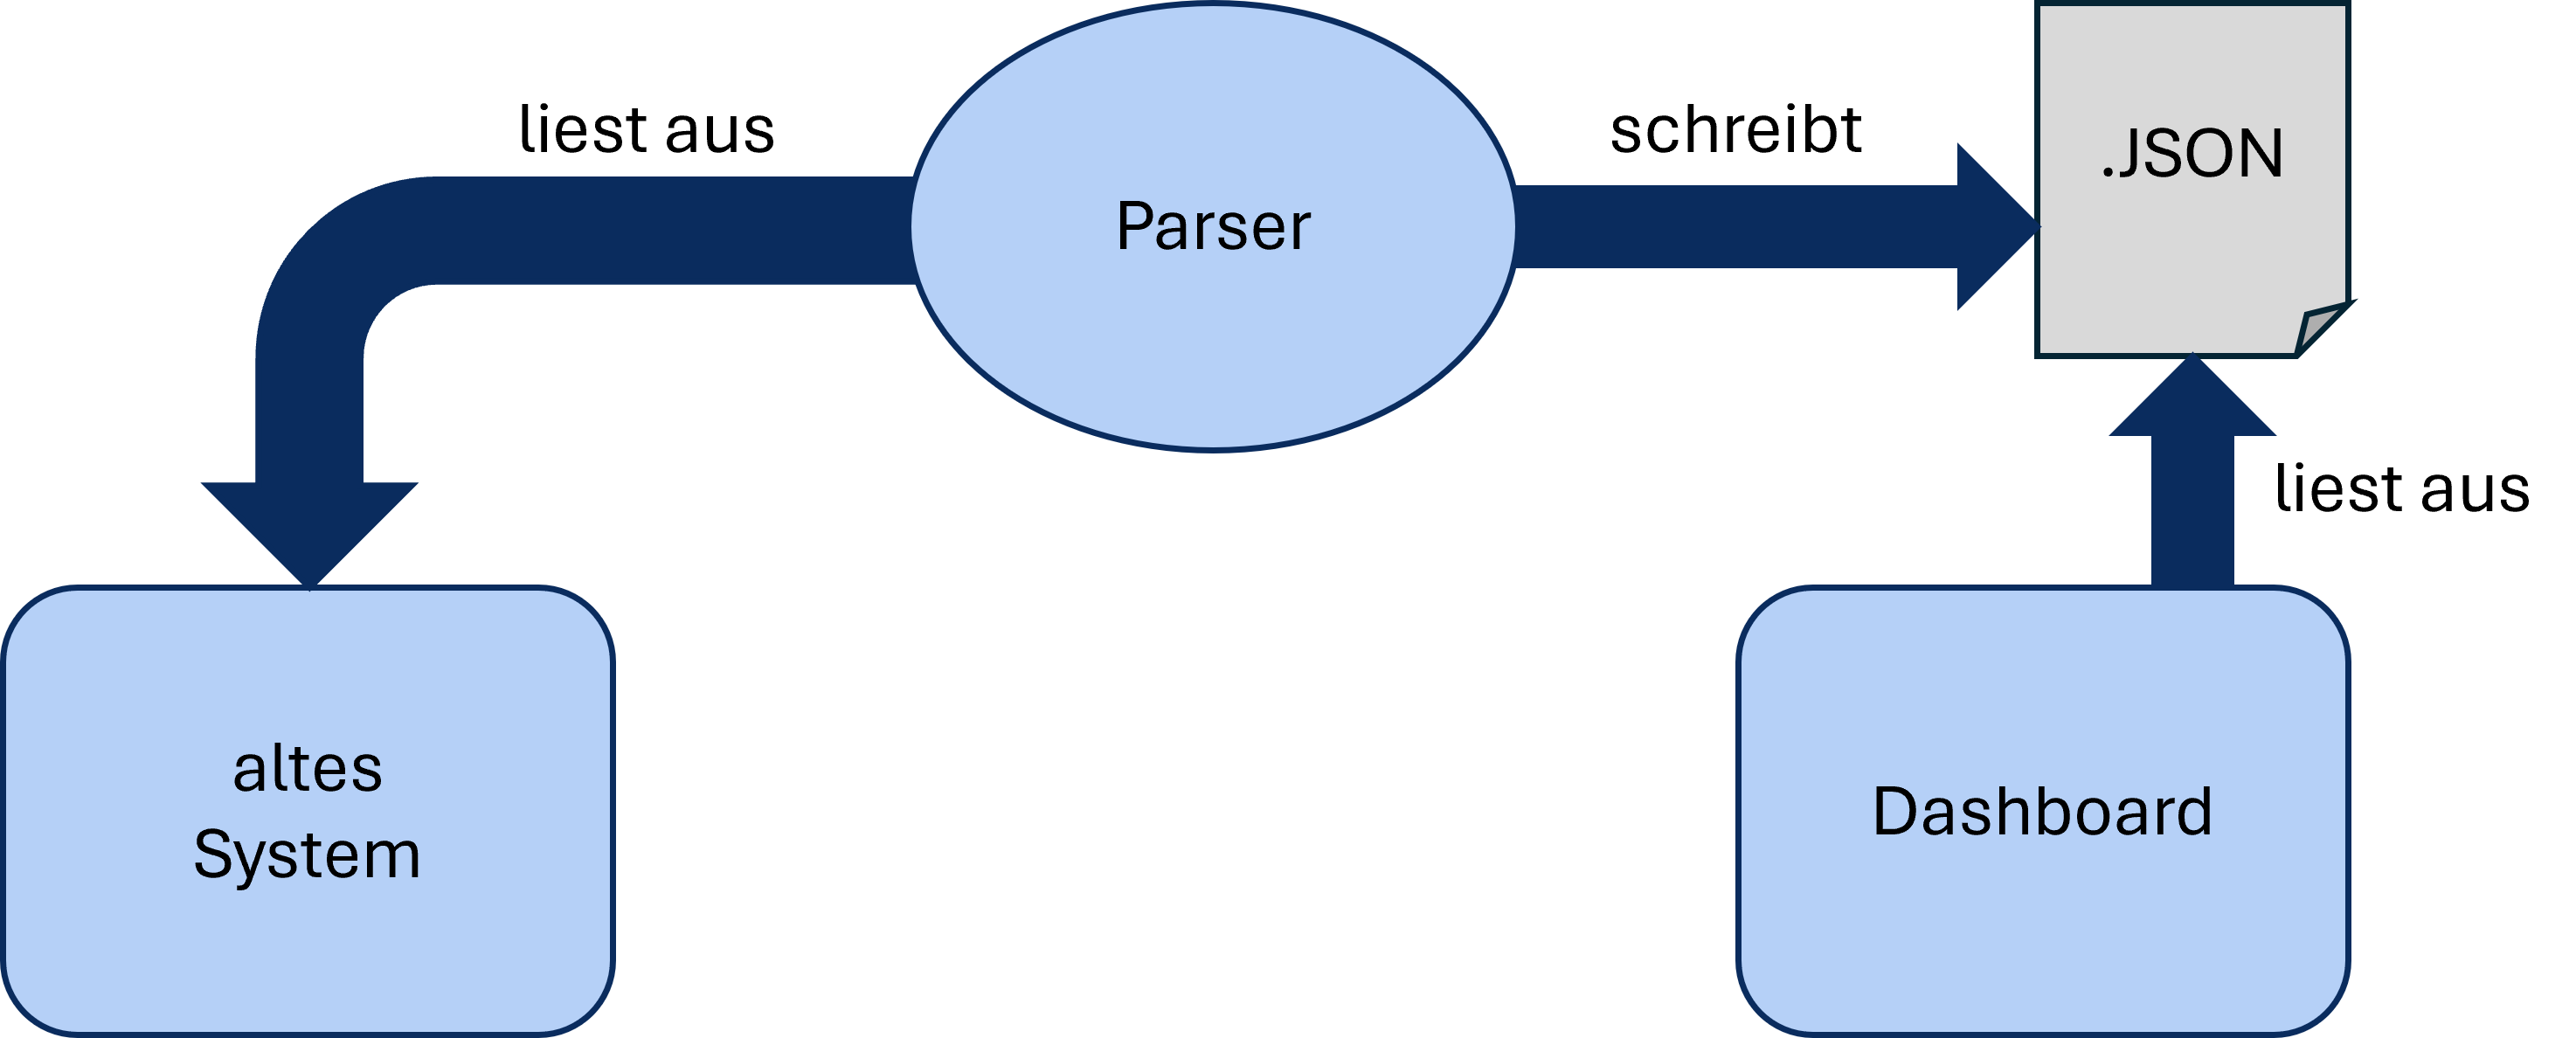
\includegraphics[width=1\linewidth]{Dashboard/Daten_Kontrollsequenz_DB.png}
    \caption{Kontrollsequenz des Datenflusses vom alten System zum Dashboard}
    \label{fig:DB_Datenfluss}
\end{figure}